\section{Campo magnético: espira circular e solenoide}

\frame{
	\frametitle{Campo magnético no centro de uma espira circular}
	\begin{block}{Introdução}
		Considere que um \textbf{fio condutor retilíneo} seja percorrido por uma corrente elétrica contínua. Considere também que esse mesmo fio seja \textbf{encurvado para formar uma espira plana circular} de raio $R$, percorrida por uma corrente elétrica de intensidade $i$.
	\end{block}
%	\vspace{0.2cm}
	
	\centering
	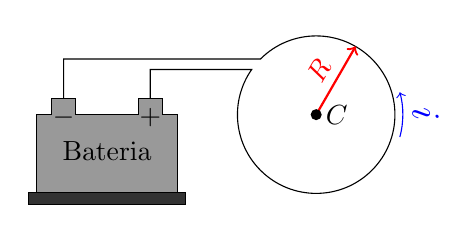
\begin{tikzpicture}
		\filldraw[fill=black!80!white] (0,0) rectangle (2,0.15);
		\filldraw[fill=black!40!white] (0.1,0.15) -- ++(0,1) -- ++(0.2,0)
		 -- ++(0,0.2) -- ++(0.15,0) node[below] {$ - $} node[coordinate,name=p1] {} -- ++(0.15,0) -- ++(0,-0.2)
		 -- ++(0.8,0)
		 -- ++(0,0.2) -- ++(0.15,0) node[below] {$ + $} node[coordinate,name=p2] {} -- ++(0.15,0) -- ++(0,-0.2)
		 -- ++(0.2,0) -- ++(0,-1) -- cycle;
		\draw[thin] (p1) -- ++(0,0.5) -- ++(2.5,0) arc(135:-215:1) node[coordinate,name=p3] {} -- (p3-|p2) -- (p2);
		\node[] at (1,0.675) {Bateria};
		\draw[red,thick,->] (p3) ++(-215:-1) node[coordinate,name=p4] {} -- node[midway,above,rotate=60] {$ R $} +(60:1);
		\draw[blue,->] (p4) ++(-15:1.1) arc(-15:15:1.1) node[midway,above,rotate=-90,blue] {\Large $ i $};
		\fill[] (p4) circle (2pt) node[right] {$ C $};
	\end{tikzpicture}
%	\centerline{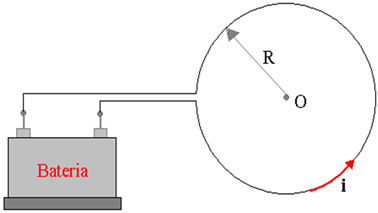
\includegraphics[width=0.6\linewidth]{Figuras/Ch08/fig1.jpg}}
}

\frame{
	\frametitle{Campo magnético no centro de uma espira circular}
	\begin{block}{Contextualização}
		Motores elétricos, transformadores, eletroímãs e outros equipamentos eletrônicos, são dispositivos que utilizam uma \textbf{bobina de fio} enrolado que cria um campo magnético com determinada finalidade.
		\begin{itemize}
			\item \textbf{Uma bobina é formada por várias espiras}.
			\item Estudaremos aqui o campo magnético formado por uma \textbf{única espira}.
		\end{itemize}
	\end{block}
}

\frame{
	\frametitle{Campo magnético no centro de uma espira circular}
	\begin{block}{Definição}
		O vetor indução magnética $\vec{B}$ no centro da espira tem as seguintes características:
		\begin{itemize}
			\item \textbf{Direção}: perpendicular ao plano da espira.
			\item \textbf{Sentido}: dado pela regra da mão direita.
			\item \textbf{Intensidade}:
			      $$\boxed{|\vec{B}| = \dfrac{\mu \cdot i}{2R}}$$
		\end{itemize}
	\end{block}
}

\frame{
	\frametitle{Campo magnético no centro de uma espira circular}
	\begin{block}{Polos da espira}
		A espira apresenta \textbf{dois pólos magnéticos}, assim como um ímã. As linhas de indução de um ímã \textbf{saem do polo norte e chegam ao polo sul}. Uma \textbf{espira} percorrida por uma corrente elétrica origina um campo magnético \textbf{análogo ao do ímã}.

		\begin{itemize}
			\item Atribui-se a espira um \textbf{polo norte, ao qual as linhas saem} (corrente circulando no sentido anti horário).
		\end{itemize}
	\end{block}
	\centerline{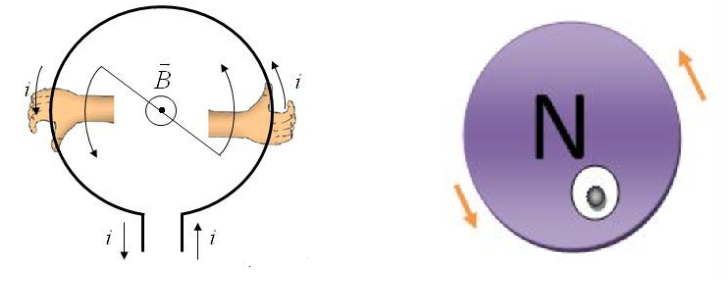
\includegraphics[width=0.7\linewidth]{Figuras/Ch08/fig2.PNG}}
}

\frame{
	\frametitle{Campo magnético no centro de uma espira circular}
	\begin{block}{Polos da espira}
		A espira apresenta \textbf{dois pólos magnéticos}, assim como um ímã. As linhas de indução de um ímã \textbf{saem do polo norte e chegam ao polo sul}. Uma \textbf{espira} percorrida por uma corrente elétrica origina um campo magnético \textbf{análogo ao do ímã}.

		\begin{itemize}
			\item Atribui-se a espira um \textbf{polo sul, ao qual as linhas chegam} (corrente circulando no sentido horário).
		\end{itemize}
	\end{block}
	\centerline{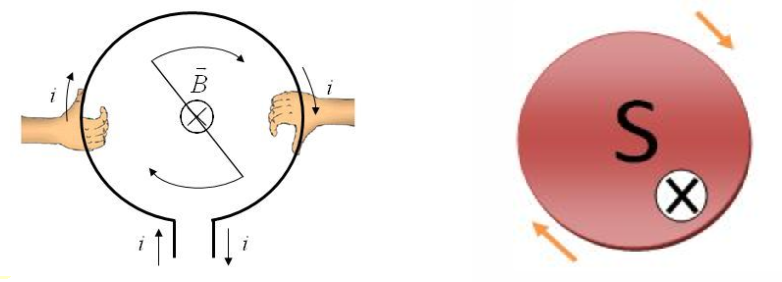
\includegraphics[width=0.7\linewidth]{Figuras/Ch08/fig3.PNG}}
}

\frame{
	\frametitle{Campo magnético no centro de uma espira circular}
	\begin{block}{Observação}
		\begin{itemize}
			\item Um observador colocado \textbf{acima da espira} vai enxergar as linhas de campo \textbf{saindo} - e essa parte representa o \textbf{polo norte}.
			\item Já quem estiver \textbf{abaixo} verá as linhas de campo \textbf{entrando} -- e essa parte representa o \textbf{polo sul}.
		\end{itemize}
	\end{block}
	\vspace{0.2cm}
	\centerline{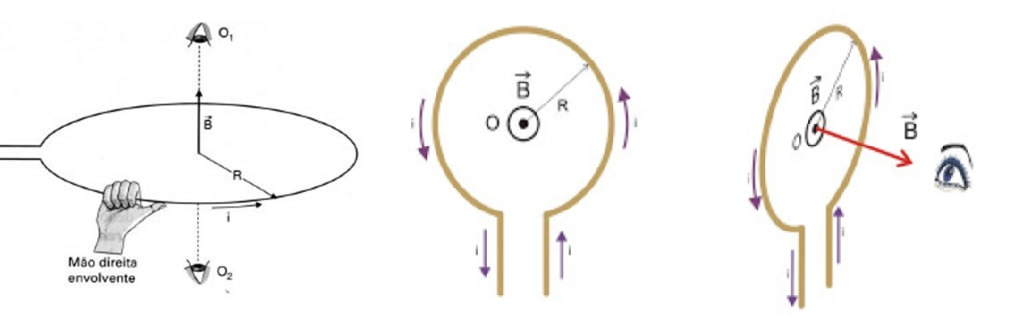
\includegraphics[width=1.1\linewidth]{Figuras/Ch08/fig4.jpg}}
}

\frame{
	\frametitle{Campo magnético no centro de uma espira circular}
	\begin{block}{Exemplo $\#01$}
		Duas espiras concêntricas e situadas num mesmo plano são percorridas pelas correntes elétricas $i_1$ e $i_2$. Sendo seus raios respectivos $R_1 = 2R$ e $R_2 = R$, qual deve ser o sentido
		da corrente $i_2$ e qual a razão entre as intensidades $i_1$ e $i_2$, para que o campo magnético resultante no centro das
		espiras seja nulo?
	\end{block}
%	\vspace{0.1cm}
	
	\centering
	\begin{tikzpicture}[x=1cm,y=1cm]
		\draw (0,0) -- ++(0,0.5) arc(-90:90:0.125) -- ++(0,0.5) arc(260:-80:1) -- ++(0,-0.5) arc(90:-90:0.125) ++(0,0.125) node[coordinate,name=p2] {} ++(0,-0.125) -- node[right] {$ i_2 $} ++(0,-0.5);
		\coordinate (p1) at (0,0.625);
		\coordinate (p3) at ($ (p1)!0.5!(p2) $);
		\draw (p3) arc(270:7:1.625) -- ++(1.125,0) node[above=0.15cm,coordinate,name=p5] {};
		\draw (p3) arc(-90:-7:1.625) -- ++(1.125,0);
		
		\coordinate (p4) at ($ (p3)+(0,1.625) $);
		\draw[dashed] (p4) -- node[midway,above,rotate=-30] {$ R_2 $} +(150:1) (p4) -- node[near end,above,rotate=60] {$ R_1 $} +(60:1.625);
		\draw[->] (p4) ++(140:1.75) arc(140:160:1.75) node[midway,above,rotate=60] {$ i_1 $};
		\draw[->] (p5) -- node[midway,above] {$ i_1 $} +(-0.5,0);
	\end{tikzpicture}
%	\centerline{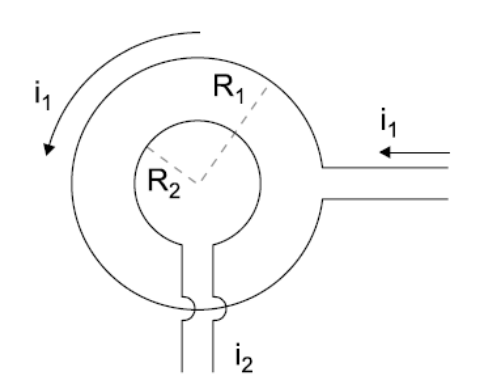
\includegraphics[width=0.6\linewidth]{Figuras/Ch08/fig6.PNG}}
}

\frame{
	\frametitle{Campo magnético no centro de uma espira circular}
	\begin{block}{Exemplo $\#01$ - Resolução}
		\begin{itemize}
			\item $|\vec{B_1}| = \dfrac{\mu \cdot i}{2R} = \dfrac{\mu \cdot i_1}{2R_1}$ (saindo do plano).
			
			\vspace{0.2cm}
			
			\item $|\vec{B_2}| = \dfrac{\mu \cdot i}{2R} = \dfrac{\mu \cdot i_2}{2R_2}$.
			
			\vspace{0.2cm}
			
			\item Para que o campo magnético resultante seja nulo, temos que ter $\vec{B_2}$ entrando no plano, de modo que se anule com $\vec{B_1}$. Desse modo:
			$$ \dfrac{\mu \cdot i_1}{2R_1} = \dfrac{\mu \cdot i_2}{2R_2} \implies \dfrac{\mu \cdot i_1}{2(2R)} = \dfrac{\mu \cdot i_2}{2(R)} \implies \dfrac{i_1}{i_2} = 2 $$
			
			\item $i_2$ possui sentido horário.
		\end{itemize}
	\end{block}
}

\frame{
	\frametitle{Campo magnético no centro de uma espira circular}
	\begin{block}{Exemplo \#02}
		Duas espiras circulares, concêntricas e coplanares de raios \SI{5\pi}{\meter} e \SI{3\pi}{\meter}, são percorridas por correntes de $i_1 = \SI{4}{\ampere} $ e $i_2 = \SI{3}{\ampere} $, como mostra a figura. Calcule o módulo do vetor indução magnética no centro das espiras.
	\end{block}
	
%	\vspace{0.5cm}
	
	\centering
	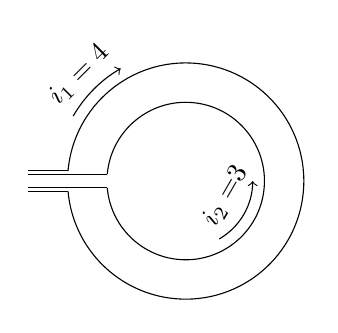
\begin{tikzpicture}[x=1cm,y=1cm]
		\draw (2,0) +(175:1) node[coordinate,name=p1] {} (2,0) +(185:1) node[coordinate,name=p2] {} (2,0) +(175:1.5) node[coordinate,name=p3] {} (2,0) +(185:1.5) node[coordinate,name=p4] {};
		\draw (p1) arc(175:-175:1) (p3) arc(175:-175:1.5);
		\foreach \x in {1,2,3,4} {
			\draw (p\x) -- (p\x -| 0,0);
		}
		\draw[->] (2,0) +(-60:0.85) arc(-60:0:0.85) node[midway,above=3pt,rotate=60] {$ i_2= $\SI{3}{\ampere}};
		\draw[<-] (2,0) +(120:1.65) arc(120:150:1.65) node[midway,above,rotate=45] {$ i_1=\SI{4}{\ampere} $};
	\end{tikzpicture}
	
%	\centerline{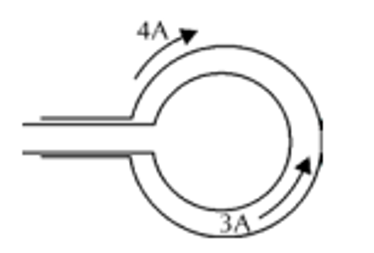
\includegraphics[width=0.5\linewidth]{Figuras/Ch08/fig7.PNG}}
}

\frame{
	\frametitle{Campo magnético no centro de uma espira circular}
	\begin{block}{Exemplo $\#02$ - Resolução}
		\begin{itemize}
			\item $|\vec{B_1}| = \dfrac{\mu \cdot i}{2R} = \dfrac{\num{4\pi e-7} \cdot 4}{2 \cdot 5\pi} = \SI{1.6e-7}{\tesla} $ (entrando no plano).
			
			\vspace{0.2cm}
			
			\item $|\vec{B_2}| = \dfrac{\mu \cdot i}{2R} = \dfrac{\num{4\pi e-7} \cdot 3}{2 \cdot 3\pi} = \SI{2e-7}{\tesla}$ (saindo do plano).
			
			\vspace{0.2cm}
			
			\item $|\vec{B_R}| = |\vec{B_2}| - |\vec{B_1}| =\SI{0.4e-7}{\tesla}$ (saindo do plano).
		\end{itemize}
	\end{block}
}

\frame{
	\frametitle{Campo magnético no centro de uma bobina chata}
	\begin{block}{Definição}
		Se considerarmos $N$ \textbf{espiras iguais justapostas}, ou seja, uma do lado da outra (em torno da mesma circunferência de raio $R$) teremos a chamada \textbf{bobina chata}.
	\end{block}
	\centerline{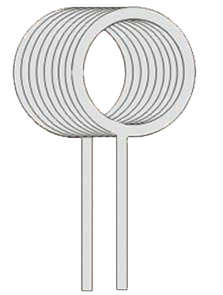
\includegraphics[width=0.3\linewidth]{Figuras/Ch08/fig5.jpg}}
}

\frame{
	\frametitle{Campo magnético no centro de uma bobina chata}
	\begin{block}{Definição}
		A intensidade do vetor indução magnética $\vec{B}$ no centro $O$ da bobina chata é determinada através da seguinte equação:
		$$\boxed{|\vec{B}| = \dfrac{N \cdot \mu \cdot i}{2R}}$$
		\begin{itemize}
			\item O sentido e a direção do vetor B da bobina é determinado da mesma maneira como na espira.
		\end{itemize}
	\end{block}
}

\frame{
	\frametitle{Campo magnético no interior de uma bobina longa (solenoide)}
	\begin{block}{Introdução}
		Solenoide é um \textbf{condutor longo} e enrolado de modo que forma um tubo constituído de \textbf{espiras igualmente espaçadas}. Aplicando uma corrente no fio, ele gera um campo magnético.
		\begin{itemize}
			\item O enrolamento de um fio sobre um tubo de caneta, por exemplo, é um solenoide. Configuramos um solenoide a partir da \textbf{reunião das configurações das linhas de campo magnético produzidas por cada uma das espiras}.
		\end{itemize}
	\end{block}

	\vspace{0.1cm}
	
	\centering
	\begin{tikzpicture}[scale=0.5,ar/.style={postaction={decorate,decoration={
		markings,mark=at position 0.5 with {\arrow{>}}
	}}}]
	% 0.3 ... how far the rings are apart
	% 0.4 ... how much from the side the rings are seen (try 0 and the same as the radius)
	% 1.5 ... radius of the rings
	\def\coil####1{
		{0.3 * (2*####1 + \t) + 0.3*sin(\t * pi r)) -0.5},
		{0.7 * cos(\t * pi r)}
	}
	
	% coil behind the rectangle
	\foreach \n in {1,2,...,4} {
		\draw[domain={0:1},smooth,variable=\t,samples=15]
		plot (\coil{\n}); 
	}
	
	\draw[domain={0:0.5},smooth,variable=\t,samples=15]
	plot (\coil{5});
	
	% Draw the rectangle
	\fill[white] (-0.5,-0.6) rectangle (3,0.6);
	\draw (-0.5,-0.6) -- ++(3.5,0) ++(0,1.2) -- ++(-3.5,0) arc(90:270:0.3 and 0.6);
	\filldraw[fill=black!40!white] (3,0) circle(0.3 and 0.6);
	
	\draw[blue, -Latex, thick] (-0.3,0) -- node[above] {$ \vec{B} $} +(3,0);
	
	% coil in front of the rectangle
	\foreach \n in {1,...,4} {
		\draw[domain={1:2},smooth,variable=\t,samples=15]
		plot (\coil{\n});
	}

	\draw[domain={1.38:2},smooth,variable=\t,samples=15]
	plot (\coil{0});
	
	\foreach \n in {0,0.6,1.2,1.8,2.4} {
		\draw[] (\n,0)+(-0.3,0.2) node[rotate=75] {<};
	}

	\draw (-0.35,-0.25) ++(-0.8pt,-0.5pt) -- +(0,-1);
	\draw[-Latex,red] (-0.45,-0.7) -- node[left] {$ i $} (-0.45,-1.15);
	
	\draw (2.8,-0.6) -- (2.8,-1.25);
	\draw[Latex-,red] (2.9,-0.7) -- node[right] {$ i $} (2.9,-1.15);
	
	\filldraw[fill=black!40!white] (-0.8,-2) -- ++(0,0.5) -- ++(0.2,0) -- ++(0,0.25) -- node[midway,below] {$ - $} ++(0.5,0) -- ++(0,-0.25) -- ++(2.65,0) -- ++(0,0.25)  -- node[midway,below] {$ + $} ++(0.5,0) -- ++(0,-0.25) -- ++(0.2,0) -- ++(0,-0.5) -- cycle;
	\node[] at (1.25,-1.75) {Bateria};
	
	\draw[dashed] (-0.5,0.6) -- +(0,0.5) (3,0.6) -- +(0,0.5);
	\draw[Latex-Latex] (-0.5,1.1) -- node[fill=white,midway] {$ L $} (3,1.1);
\end{tikzpicture}
	
%	\centerline{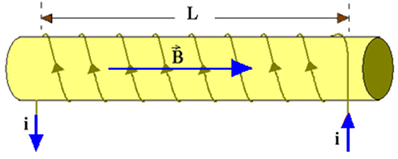
\includegraphics[width=0.65\linewidth]{Figuras/Ch08/fig8.jpg}}
}

\frame{
	\frametitle{Campo magnético no interior de uma bobina longa (solenoide)}
	\begin{block}{Definição}
		O vetor indução magnética $\vec{B}$ no interior de um solenoide tem as seguintes características:
		\begin{itemize}
			\item \textbf{Direção}: retilínea e paralela ao eixo do solenoide.
			\item \textbf{Sentido}: obtido através da regra da mão direita.
			\item \textbf{Intensidade}:
			      $$\boxed{|\vec{B}| = \dfrac{N \cdot \mu \cdot i}{L}}$$
		\end{itemize}
	\end{block}
}

\frame{
	\frametitle{Campo magnético no interior de uma bobina longa (solenoide)}
	\begin{block}{Observações}
		\begin{itemize}
			\item O campo do solenoide é bem semelhante ao campo de um ímã em forma de barra, onde a extremidade por onde saem as linhas de campo é o polo norte, e a extremidade por onde entram as linhas de campo é o polo sul.
		\end{itemize}
	\end{block}
	\centerline{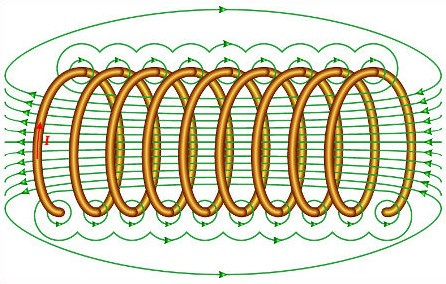
\includegraphics[width=0.55\linewidth]{Figuras/Ch08/fig9.jpg}}
}

\frame{
	\frametitle{Campo magnético no interior de uma bobina longa (solenoide)}
	\begin{block}{Observações}
		\begin{itemize}
			\item As espiras que estão na parte \textbf{de cima do desenho apresentam campos magnéticos com sentidos contrários aos das que estão na parte de baixo}, devido ao sentido da corrente, que é invertida. Assim, os campos das espiras de cima anulam o efeito dos campos das espiras de baixo. E, dessa forma, teremos um \textbf{campo magnético resultante nulo na parte externa do solenoide}.
		\end{itemize}
	\end{block}
	\centerline{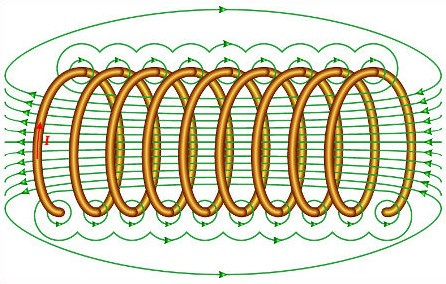
\includegraphics[width=0.55\linewidth]{Figuras/Ch08/fig9.jpg}}
}

\frame{
	\frametitle{Campo magnético no interior de uma bobina longa (solenoide)}
	\begin{block}{Observações}
		\begin{itemize}
			\item No \textbf{interior do solenoide} consideramos o \textbf{campo magnético como sendo uniforme}, portanto, \textbf{as linhas de indução são paralelas entre si}. Quanto mais comprido for o solenoide, mais uniforme será o campo magnético interno e mais fraco o campo magnético externo.
		\end{itemize}
	\end{block}
	\centerline{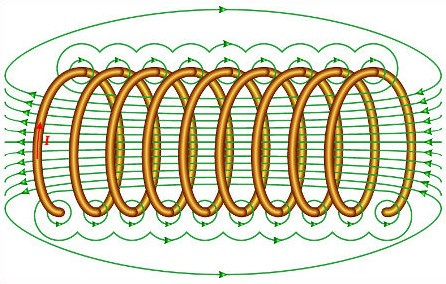
\includegraphics[width=0.55\linewidth]{Figuras/Ch08/fig9.jpg}}
}

\frame{
	\frametitle{Campo magnético no interior de um solenoide}
	\begin{block}{Exemplo $\#01$}
		A figura representa uma bateria, de força eletromotriz $E$ e resistência interna $R = \SI{5}{\ohm}$, ligada a um solenoide de 200 espiras. Sabe-se que o amperímetro marca \SI{200}{\milli\ampere} e o voltímetro marca \SI{8.0}{\volt}, ambos supostos ideais. (a) Qual o valor da força eletromotriz da bateria? (b) Qual a intensidade do campo magnético gerado no ponto $ P $, localizado no meio do interior vazio do solenoide?
	\end{block}
	
%	\vspace{0.1cm}
	
	\centering
	\begin{circuitikz}[scale=0.9]
		\draw (0,0) to[battery,l=$ \epsilon $, *-] ++(1,0)
		to[R=5<\ohm>,l=$ R $, -*] ++(1,0)
		to[rmeter,t=A] ++(0,1)
		to[L] ++(-2,0)
		-- ++(0,-1.4)
		to[rmeter,t=V] ++(2,0)
		-- ++(0,0.4);
		\draw[dashed] (0.77,1.25) -- +(0,-0.25) (1.23,1.25) -- +(0,-0.25);
		\draw[<->] (0.77,1.2) -- node[midway,above=1pt] {\SI{20}{\centi\meter}} +(0.46,0);
		\draw[-Latex] (1,0.65) -- node[midway,left] {$ P $} +(0,0.2);
	\end{circuitikz}
	
%	\centerline{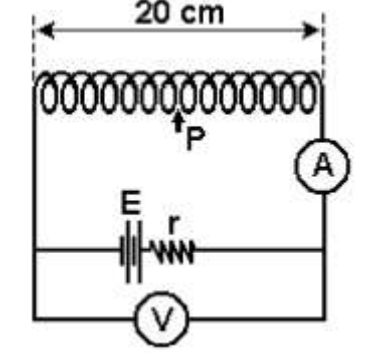
\includegraphics[width=0.4\linewidth]{Figuras/Ch08/fig10.PNG}}
}

\frame{
	\frametitle{Campo magnético no centro de uma espira circular}
	\begin{block}{Exemplo $\#01$ - Resolução}
		\begin{enumerate}[(a)]
			\item $V_r = R \cdot I = 5 \cdot \num{0,2} = \SI{1}{\volt}$. \\
			      Temos que $V = \epsilon - V_r \therefore \epsilon = V + V_r = 8 + 1 = \SI{9}{\volt}$
			      
			\vspace{0.2cm}
			\item $|\vec{B}| = \dfrac{N \cdot \mu \cdot i}{L} = \dfrac{200 \cdot \num{4\pi e-7} \cdot \num{0,2}}{\num{0,2}} = \SI{2.51e-4}{\tesla}$
		\end{enumerate}
	\end{block}
}

\section*{Exercícios}
\frame{
	\frametitle{Exercícios}
	\begin{block}{}
		01. (PUC-RS) Para uma espira circular condutora, percorrida por uma corrente elétrica de intensidade $i$, é registrado um campo magnético de intensidade $|\vec{B}|$ no seu centro. Alterando-se a intensidade da corrente elétrica na espira para um novo valor $i_{\text{final}}$, observa-se que o módulo do campo magnético, no mesmo ponto, assumirá o valor $5|\vec{B}|$. Qual é a razão entre as intensidades das correntes elétricas final ($i_{\text{final}}$) e inicial ($i$)?

		\vspace{0.5cm}

		02. Considere dois solenoides, o primeiro com um número de espiras $N_1 = 120$, de comprimento $L_1 = \SI{30}{\centi\meter} $, e o segundo com $N_2 = 180$ espiras e um comprimento $L_2 = \SI{15}{\centi\meter} $. O primeiro é percorrido por uma corrente $i_1 = \SI{6}{\ampere} $. Qual é a corrente $i_2$ que devemos fazer passar no segundo para que o campo magnético seja o mesmo no interior dos dois solenoides?
	\end{block}
}

\section*{Referências}
\frame{
	\frametitle{Referências e Exercícios Complementares}
	\begin{itemize}
		\item ALEXANDRE, Charles K.; SADIKU, Matthew N. O. Fundamentos de Circuitos Elétricos. 5. ed. Porto Alegre: AMGH, 2013.
	\end{itemize}
	%\centering{\alert{Página 36 - \textbf{1.6.1 até 1.6.5, 1.6.17 até 1.6.19}}} \\
	\centering{\alert{Lista de exercícios 08}}
}